\subsection*{Первое задание}
Нам нужно доказать, что
\begin{equation*}
	\ket{n} = \frac{(a\con)^n}{\sqrt{n!}} \ket{0}.
\end{equation*}
Действительно (по 17 слайду презентации например)
\begin{equation*}
	\bk{n}[a a\con]{n} = \bk{n}[[a, a\con]+ a\con a]{n} = \bk{n}[N+1]{n} = n+1.
\end{equation*}
A значит
\begin{equation*}
	a\con \ket{n} = \sqrt{n+1} \ket{n+1},
\end{equation*}
наконец
\begin{equation*}
	\ket{n} = \frac{a\con}{\sqrt{n}} \ket{n-1} = \frac{(a\con)^2}{\sqrt{n(n-1)}} \ket{n-2} = \cdots = \frac{(a\con)^n}{\sqrt{n!}} \ket{0}.
\end{equation*}

\subsection*{Второе задание}
    \begin{figure}[htb]
    \centering
    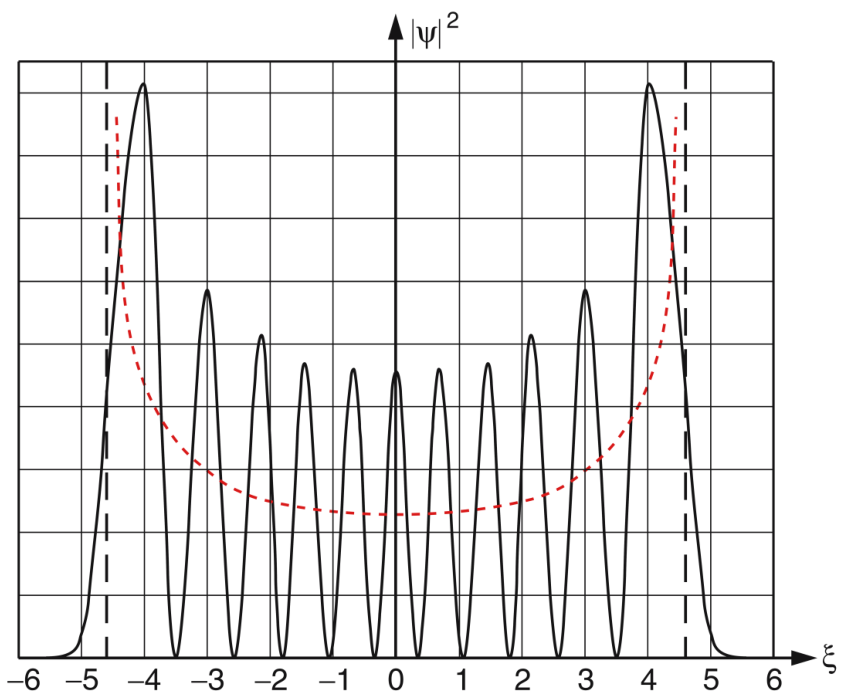
\includegraphics[width=0.5\textwidth]{img/lohmanscay_osc2.png}
    \caption{Тут всё просто --- $n = 10$.}
    %\label{fig:}
\end{figure}
    


\subsection*{Третье задание}
И так мы знаем, что 
\begin{equation*}
	a(t) = a(0) e^{i \omega t},
	\hspace{1 cm}
	a\con(t) = a\con(0) e^{i \omega t}.
\end{equation*}
Знаем, уравнения эволюции системы:
\begin{equation*}
	\frac{d p }{d t} = - \frac{\partial}{\partial x} V(x),
	\hspace{1 cm}
	 \frac{d x}{d t} = \frac{p}{m}.
\end{equation*}
Где $V$ -- возмущения в нашем гамильтониане:
\begin{equation*}
	H = \frac{p^2}{2 m} + V(x) = \frac{p^2}{2 m} + \frac{m \omega^2 x^2}{2}.
\end{equation*}
То есть получаем:
\begin{equation*}
	\frac{d p }{d t} = - m \omega^2 x
	\hspace{1 cm}
	\frac{d x}{d t} = \frac{p}{m}.
\end{equation*}
Теперь заметим, что для $a$ определенных как:
\begin{equation*}
	a = \sqrt{\frac{m \omega}{2 \hbar}} \left(x + \frac{i p }{m \omega}\right),
	\hspace{1 cm}
	a\con = \sqrt{\frac{m \omega}{2 \hbar}} \left(x - \frac{i p }{m \omega}\right).
\end{equation*}
Мы из наших уравнений на $x$ и $p$ как раз и имеем:
\begin{equation*}
	\frac{d a}{d t} = \sqrt{\frac{m \omega}{2 \hbar}\left(\frac{p}{m} - i \omega x\right)} = - i \omega a
	\hspace{1 cm}
	\Rightarrow
	\hspace{1 cm}
	a(t) = a(0) e^{- i \omega t}
\end{equation*}
Аналогично для сопряженной $a\con = a\con(0) e^{i \omega t}$.

Тогда просто подставим $a$ по определению через $x$ и $p$:
\begin{equation*}
	\left.
	\begin{aligned}
		x(t) + \frac{i p (t)}{m \omega} = x(0) \exp(-i\omega t) + i \left(\frac{p(0)}{m \omega}\right) e^{- i \omega t}\\
		x(t) - \frac{i p (t)}{m \omega} = x(0) \exp(-i\omega t) - i \left(\frac{p(0)}{m \omega}\right) e^{i \omega t}
	\end{aligned}
	\right\}
	+
	\hspace{0.3 cm}
	\Rightarrow
\end{equation*}
\begin{equation*}
	x(t) = x(0) \cos \omega t + \left(\frac{p(0)}{m \omega}\right) \sin \omega t.
\end{equation*}
Что и требовалось вывести.